\documentclass[
  man,
  floatsintext,
  longtable,
  a4paper,
  nolmodern,
  notxfonts,
  notimes,
  colorlinks=true,linkcolor=blue,citecolor=blue,urlcolor=blue]{apa7}

\usepackage{amsmath}
\usepackage{amssymb}




\RequirePackage{longtable}
\RequirePackage{threeparttablex}

\makeatletter
\renewcommand{\paragraph}{\@startsection{paragraph}{4}{\parindent}%
	{0\baselineskip \@plus 0.2ex \@minus 0.2ex}%
	{-.5em}%
	{\normalfont\normalsize\bfseries\typesectitle}}

\renewcommand{\subparagraph}[1]{\@startsection{subparagraph}{5}{0.5em}%
	{0\baselineskip \@plus 0.2ex \@minus 0.2ex}%
	{-\z@\relax}%
	{\normalfont\normalsize\bfseries\itshape\hspace{\parindent}{#1}\textit{\addperi}}{\relax}}
\makeatother




\usepackage{longtable, booktabs, multirow, multicol, colortbl, hhline, caption, array, float, xpatch}
\usepackage{subcaption}


\renewcommand\thesubfigure{\Alph{subfigure}}
\setcounter{topnumber}{2}
\setcounter{bottomnumber}{2}
\setcounter{totalnumber}{4}
\renewcommand{\topfraction}{0.85}
\renewcommand{\bottomfraction}{0.85}
\renewcommand{\textfraction}{0.15}
\renewcommand{\floatpagefraction}{0.7}

\usepackage{tcolorbox}
\tcbuselibrary{listings,theorems, breakable, skins}
\usepackage{fontawesome5}

\definecolor{quarto-callout-color}{HTML}{909090}
\definecolor{quarto-callout-note-color}{HTML}{0758E5}
\definecolor{quarto-callout-important-color}{HTML}{CC1914}
\definecolor{quarto-callout-warning-color}{HTML}{EB9113}
\definecolor{quarto-callout-tip-color}{HTML}{00A047}
\definecolor{quarto-callout-caution-color}{HTML}{FC5300}
\definecolor{quarto-callout-color-frame}{HTML}{ACACAC}
\definecolor{quarto-callout-note-color-frame}{HTML}{4582EC}
\definecolor{quarto-callout-important-color-frame}{HTML}{D9534F}
\definecolor{quarto-callout-warning-color-frame}{HTML}{F0AD4E}
\definecolor{quarto-callout-tip-color-frame}{HTML}{02B875}
\definecolor{quarto-callout-caution-color-frame}{HTML}{FD7E14}

%\newlength\Oldarrayrulewidth
%\newlength\Oldtabcolsep


\usepackage{hyperref}




\providecommand{\tightlist}{%
  \setlength{\itemsep}{0pt}\setlength{\parskip}{0pt}}
\usepackage{longtable,booktabs,array}
\usepackage{calc} % for calculating minipage widths
% Correct order of tables after \paragraph or \subparagraph
\usepackage{etoolbox}
\makeatletter
\patchcmd\longtable{\par}{\if@noskipsec\mbox{}\fi\par}{}{}
\makeatother
% Allow footnotes in longtable head/foot
\IfFileExists{footnotehyper.sty}{\usepackage{footnotehyper}}{\usepackage{footnote}}
\makesavenoteenv{longtable}

\usepackage{graphicx}
\makeatletter
\newsavebox\pandoc@box
\newcommand*\pandocbounded[1]{% scales image to fit in text height/width
  \sbox\pandoc@box{#1}%
  \Gscale@div\@tempa{\textheight}{\dimexpr\ht\pandoc@box+\dp\pandoc@box\relax}%
  \Gscale@div\@tempb{\linewidth}{\wd\pandoc@box}%
  \ifdim\@tempb\p@<\@tempa\p@\let\@tempa\@tempb\fi% select the smaller of both
  \ifdim\@tempa\p@<\p@\scalebox{\@tempa}{\usebox\pandoc@box}%
  \else\usebox{\pandoc@box}%
  \fi%
}
% Set default figure placement to htbp
\def\fps@figure{htbp}
\makeatother


% definitions for citeproc citations
\NewDocumentCommand\citeproctext{}{}
\NewDocumentCommand\citeproc{mm}{%
  \begingroup\def\citeproctext{#2}\cite{#1}\endgroup}
\makeatletter
 % allow citations to break across lines
 \let\@cite@ofmt\@firstofone
 % avoid brackets around text for \cite:
 \def\@biblabel#1{}
 \def\@cite#1#2{{#1\if@tempswa , #2\fi}}
\makeatother
\newlength{\cslhangindent}
\setlength{\cslhangindent}{1.5em}
\newlength{\csllabelwidth}
\setlength{\csllabelwidth}{3em}
\newenvironment{CSLReferences}[2] % #1 hanging-indent, #2 entry-spacing
 {\begin{list}{}{%
  \setlength{\itemindent}{0pt}
  \setlength{\leftmargin}{0pt}
  \setlength{\parsep}{0pt}
  % turn on hanging indent if param 1 is 1
  \ifodd #1
   \setlength{\leftmargin}{\cslhangindent}
   \setlength{\itemindent}{-1\cslhangindent}
  \fi
  % set entry spacing
  \setlength{\itemsep}{#2\baselineskip}}}
 {\end{list}}
\usepackage{calc}
\newcommand{\CSLBlock}[1]{\hfill\break\parbox[t]{\linewidth}{\strut\ignorespaces#1\strut}}
\newcommand{\CSLLeftMargin}[1]{\parbox[t]{\csllabelwidth}{\strut#1\strut}}
\newcommand{\CSLRightInline}[1]{\parbox[t]{\linewidth - \csllabelwidth}{\strut#1\strut}}
\newcommand{\CSLIndent}[1]{\hspace{\cslhangindent}#1}





\usepackage{newtx}

\defaultfontfeatures{Scale=MatchLowercase}
\defaultfontfeatures[\rmfamily]{Ligatures=TeX,Scale=1}





\title{A Poisson Count Race as a Generative Bridge Between Logit and
Probit Choice}


\shorttitle{Poisson count race unifies logit and probit}


\usepackage{etoolbox}






\author{Vencislav Popov}



\affiliation{
{Department of Psychology, University of Zurich}}




\leftheader{Popov}



\abstract{This study unifies the two canonical discrete choice
specifications - multinomial logit and multinomial probit - within a
single count process. The model uses a Poisson count process race,
wherein \(K\) alternatives generate events according to independent
Poisson processes. A choice is determined when an alternative reaches a
cumulative count threshold \(\theta\). At the single-event threshold,
\(\theta=1\), the model yields the Multinomial Logit (Luce choice rule).
By normalizing the utility noise to maintain a constant variance, I show
that as \(\theta \to \infty\), the model converges to the Multinomial
Probit. This formulation provides a parametric bridge in which
\(\theta\) governs the shape of the error distribution and a separate
parameter, \(\beta\), modulates the variance, while the systematic
utilities \(v_i\) are shared across all regimes. The generalized model
uses a single stochastic accumulation mechanism: both regimes belong to
the log-Gamma random utility family, with \(\theta\) governing the
transition between Gumbel and Gaussian noise shapes. The unification is
distributional rather than dynamical: changes in \(\theta\) do not
represent a single decision-making system adjusting its threshold in
real time, but rather compare different accumulation regimes at matched
discriminability. }

\keywords{discrete choice, random utility, multinomial
logit, multinomial probit, Poisson process, evidence accumulation}

\authornote{\par{\addORCIDlink{Vencislav Popov}{0000-0002-8073-4199}} 

\par{       }
\par{Correspondence concerning this article should be addressed
to Vencislav
Popov, Email: \href{mailto:vencislav.popov@gmail.com}{vencislav.popov@gmail.com}}
}

\makeatletter
\let\endoldlt\endlongtable
\def\endlongtable{
\hline
\endoldlt
}
\makeatother

\urlstyle{same}



\makeatletter
\@ifpackageloaded{tcolorbox}{}{\usepackage[skins,breakable]{tcolorbox}}
\@ifpackageloaded{fontawesome5}{}{\usepackage{fontawesome5}}
\definecolor{quarto-callout-color}{HTML}{909090}
\definecolor{quarto-callout-note-color}{HTML}{0758E5}
\definecolor{quarto-callout-important-color}{HTML}{CC1914}
\definecolor{quarto-callout-warning-color}{HTML}{EB9113}
\definecolor{quarto-callout-tip-color}{HTML}{00A047}
\definecolor{quarto-callout-caution-color}{HTML}{FC5300}
\definecolor{quarto-callout-color-frame}{HTML}{acacac}
\definecolor{quarto-callout-note-color-frame}{HTML}{4582ec}
\definecolor{quarto-callout-important-color-frame}{HTML}{d9534f}
\definecolor{quarto-callout-warning-color-frame}{HTML}{f0ad4e}
\definecolor{quarto-callout-tip-color-frame}{HTML}{02b875}
\definecolor{quarto-callout-caution-color-frame}{HTML}{fd7e14}
\makeatother
\makeatletter
\@ifpackageloaded{caption}{}{\usepackage{caption}}
\AtBeginDocument{%
\ifdefined\contentsname
  \renewcommand*\contentsname{Table of contents}
\else
  \newcommand\contentsname{Table of contents}
\fi
\ifdefined\listfigurename
  \renewcommand*\listfigurename{List of Figures}
\else
  \newcommand\listfigurename{List of Figures}
\fi
\ifdefined\listtablename
  \renewcommand*\listtablename{List of Tables}
\else
  \newcommand\listtablename{List of Tables}
\fi
\ifdefined\figurename
  \renewcommand*\figurename{Figure}
\else
  \newcommand\figurename{Figure}
\fi
\ifdefined\tablename
  \renewcommand*\tablename{Table}
\else
  \newcommand\tablename{Table}
\fi
}
\@ifpackageloaded{float}{}{\usepackage{float}}
\floatstyle{ruled}
\@ifundefined{c@chapter}{\newfloat{codelisting}{h}{lop}}{\newfloat{codelisting}{h}{lop}[chapter]}
\floatname{codelisting}{Listing}
\newcommand*\listoflistings{\listof{codelisting}{List of Listings}}
\makeatother
\makeatletter
\makeatother
\makeatletter
\@ifpackageloaded{caption}{}{\usepackage{caption}}
\@ifpackageloaded{subcaption}{}{\usepackage{subcaption}}
\makeatother

% From https://tex.stackexchange.com/a/645996/211326
%%% apa7 doesn't want to add appendix section titles in the toc
%%% let's make it do it
\makeatletter
\xpatchcmd{\appendix}
  {\par}
  {\addcontentsline{toc}{section}{\@currentlabelname}\par}
  {}{}
\makeatother

%% Disable longtable counter
%% https://tex.stackexchange.com/a/248395/211326

\usepackage{etoolbox}

\makeatletter
\patchcmd{\LT@caption}
  {\bgroup}
  {\bgroup\global\LTpatch@captiontrue}
  {}{}
\patchcmd{\longtable}
  {\par}
  {\par\global\LTpatch@captionfalse}
  {}{}
\apptocmd{\endlongtable}
  {\ifLTpatch@caption\else\addtocounter{table}{-1}\fi}
  {}{}
\newif\ifLTpatch@caption
\makeatother

\begin{document}

\maketitle



\setcounter{secnumdepth}{3}

\setlength\LTleft{0pt}




\textsubscript{Source:
\href{https://venpopov.github.io/logit-probit-poisson-rum/index.qmd.html}{Article
Notebook}}

\section{Introduction}\label{introduction}

Discrete choice models based on Random Utility (RU) theory
(\citeproc{ref-mcfaddenConditionalLogitAnalysis1974}{McFadden, 1974})
form a central pillar of mathematical psychology, econometrics, and
cognitive science. In these models, each alternative in a choice set
elicits a \emph{latent} scalar quantity - often interpreted as strength,
utility, or evidence - and the observed choices arise from a comparison
of these latent quantities under stochastic variability. The general
setup is surprisingly simple. Consider a decision-maker facing a set of
\(K \ge 2\) mutually exclusive alternatives. The utility associated with
alternative \(i\) can be decomposed into a systematic component,
\(v_i\), and a stochastic component, \(\epsilon_i\):

\[
U_{i} = v_{i} + \epsilon_{i}, \quad i=1, \dots, K
\]

The decision-maker then selects the alternative with maximum utility:

\[
C = \arg \max_{i \in K} U_{i}
\]

While the term ``utility'' implies an economic setting, the underlying
mathematical model concerns any situation in which choices are
probabilistic. The core concept is that of a shared \emph{random scale}
on which multiple latent variables, each associated with a different
choice, are represented. Any choice model that implements this
assumption, together with the max choice rule, is said to have a
random-scale representation or to be random-scale representible
(\citeproc{ref-falmagneRepresentationTheoremFinite1978a}{Falmagne,
1978}; \citeproc{ref-kellenTestingFoundationsSignal2021}{Kellen et al.,
2021}).

Within this general framework, different assumptions about the
distribution of errors, \(\epsilon_i\), determine the structure of the
choice model and its predictions. Two important classes dominate the
field: logit-based models, derived from Luce's choice axiom and
extreme-value theory
(\citeproc{ref-luceIndividualChoiceBehavior1959}{Luce, 1959};
\citeproc{ref-mcfaddenConditionalLogitAnalysis1974}{McFadden, 1974};
\citeproc{ref-yellottRelationshipLucesChoice1977}{Yellott, 1977}), and
probit-based models, derived from Thurstone's Theory of comparative
judgements and gaussian Signal Detection Theory
(\citeproc{ref-hausmanConditionalProbitModel1978a}{Hausman \& Wise,
1978}; \citeproc{ref-robinsonHowPeopleBuild2023}{Robinson et al., 2023};
\citeproc{ref-thurstoneLawComparativeJudgment1927}{Thurstone, 1927};
\citeproc{ref-wixtedForgottenHistorySignal2020}{Wixted, 2020}). These
two model families correspond to two types of error distributions:

\begin{enumerate}
\def\labelenumi{\arabic{enumi}.}
\item
  \textbf{Gumbel Errors:} If the \(\epsilon_i\) terms are independent
  and identically distributed (i.i.d.) according to a Type I Extreme
  Value distribution, the choice probabilities follow the
  \textbf{Multinomial Logit (MNL)} or Softmax form.
\item
  \textbf{Gaussian Errors:} If the \(\epsilon_i\) terms follow a
  Multivariate Normal distribution (potentially allowing for correlated
  errors across alternatives) the choice probabilities are described by
  the \textbf{Multinomial Probit (MNP)} model.
\end{enumerate}

\phantomsection\label{cell-fig-rum-overview}
\begin{figure}[H]

\caption{\label{fig-rum-overview}The two canonical random utility
models. Left panels show the noise distributions for each alternative,
with a single random draw from each (the winning draw is highlighted).
Right panels show the corresponding choice probability formulas. Top
row: Gumbel (Type I Extreme Value) noise yields the Multinomial Logit
(Softmax). Bottom row: Gaussian noise yields the Multinomial Probit.}

\centering{

\pandocbounded{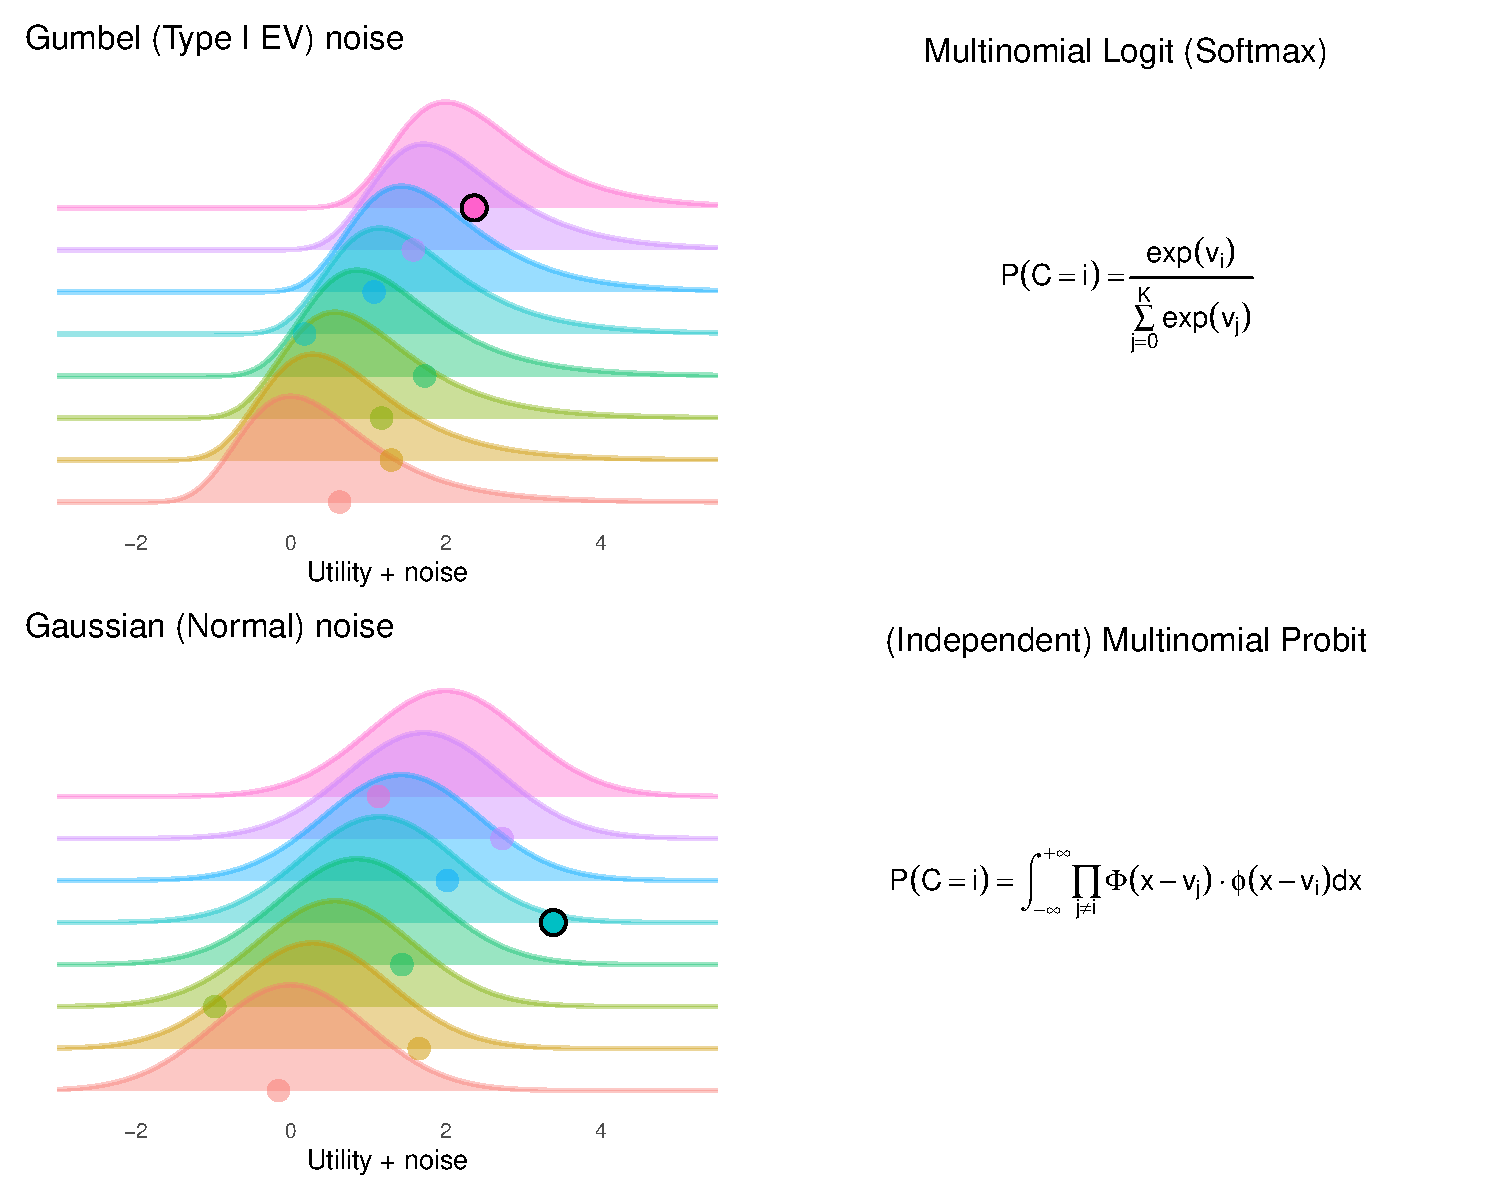
\includegraphics[keepaspectratio]{index_files/figure-pdf/fig-rum-overview-1.pdf}}

}

\end{figure}%

\textsubscript{Source:
\href{https://venpopov.github.io/logit-probit-poisson-rum/index.qmd.html}{Article
Notebook}}

The random utility framework thus unifies axiomatic choice models
(\citeproc{ref-luceIndividualChoiceBehavior1959}{Luce, 1959}) and
measurement detection-based models
(\citeproc{ref-thurstoneLawComparativeJudgment1927}{Thurstone, 1927})
under a single functional form. However, the unification currently stops
there - the different error distributions reflect different assumptions
about the generating process. As Robinson et al.
(\citeproc{ref-robinsonHowPeopleBuild2023}{2023}) recently put it, the
two models ``describe different ways of translating sensory evidence
into decision variables.''.

The central question addressed in this paper is this: Can the two
canonical random-utility discrete-choice specifications --- multinomial
logit and multinomial probit --- be derived from a shared generative
mechanism? Can we find a deeper unifying principle? The surprising
answer is yes - both models can be derived as limit cases of a single
stochastic evidence accumulation mechanism. The key distinction between
the models is not the form of the utility noise itself, but the stopping
rule governing how stochastic evidence is accumulated before a choice is
made.

\subsection{Model overview}\label{model-overview}

Take a \textbf{Poisson count race}
(\citeproc{ref-pikeResponseLatencyModels1973}{Pike, 1973};
\citeproc{ref-smithTimedependentPoissonCounter2000a}{Smith \& Van Zandt,
2000}; \citeproc{ref-townsendStochasticModelingElementary1983}{Townsend
\& Ashby, 1983}), wherein each alternative generates stochastic events
via an independent Poisson process. A decision is made when one
alternative reaches a cumulative count threshold \(\theta\). The
threshold \(\theta\) thus controls how much stochastic evidence must be
accumulated before commitment.

Without any additional modifications, such a model predicts increasingly
deterministic responses, and in the limit as \(\theta \to \infty\) it
leads to choosing the option with the highest utility 100\% of the time.
To prevent this, and to compare noise \emph{shape} across \(\theta\)
independently of noise \emph{scale}, we must standardize the stochastic
utility component to unit variance for all \(\theta\), with a separate
parameter \(\beta\) controlling the overall magnitude of stochasticity.
With this normalization, we can establish three main results:

\begin{enumerate}
\def\labelenumi{\arabic{enumi}.}
\tightlist
\item
  At \(\theta = 1\), this reduces exactly to the Multinomial Logit
\item
  For any \(\theta \ge 1\), the Poisson count race is isomorphic to a
  random utility model with log-Gamma noise, interpolating between
  Gumbel and Gaussian error distributions;
\item
  As \(\theta \to \infty\) the model converges to the Multinomial
  Probit.
\end{enumerate}

From this perspective, logit and probit can be understood as members of
a single parametric family of evidence accumulation models that differ
in the accumulation stopping rule. Extreme-value noise and Gaussian
noise arise as the two endpoint regimes of log-Gamma noise, which is the
natural error distribution of Poisson count races. It is important to
note, however, that this unification is algebraic and distributional
rather than dynamical: the standartization that enables comparison
across \(\theta\) values compares different accumulation systems at
matched discriminability, not a single system under threshold variation
(see Section 5 for details).

While Poisson counter models have a rich history in mathematical
psychology---particularly as accounts of response time distributions
under time-varying evidence rates
(\citeproc{ref-pikeResponseLatencyModels1973}{Pike, 1973};
\citeproc{ref-smithTimedependentPoissonCounter2000a}{Smith \& Van Zandt,
2000}; \citeproc{ref-townsendStochasticModelingElementary1983}{Townsend
\& Ashby, 1983}) - they have rarely been invoked to address the
theoretical relationship between \emph{static} discrete choice models.
For example, Smith and Van Zandt (2000) showed that Poisson races yield
choice probabilities governed by the incomplete Beta function when there
are two options to choose from; but their analysis focused on relatively
small integer thresholds \(\theta \approx 5\text{–}10\) chosen to
capture reaction-time skewness.

The present work takes a different perspective. Rather than treating the
threshold as a fixed descriptive parameter, I examine the asymptotic
behavior of the Poisson count race as \(\theta \to \infty\) under
variance-preserving identification. This shift in emphasis reveals that
the Poisson race is not merely a model of latency, but a generative
mechanism that continuously interpolates between the two canonical
pillars of discrete choice: Multinomial Logit \(\theta = 1\) and
Multinomial Probit \(\theta \to \infty\).

The remainder of the paper formalizes this framework, presents
simulations illustrating the interpolation between regimes, and
discusses implications for discrete choice modeling.

\section{The Generative Model: A Poisson Count
Race}\label{the-generative-model-a-poisson-count-race}

Let the accumulation of evidence or preference for each alternative
\(i\) be modeled by independent Poisson count processes, denoted
\(N_i(t)\), with rate parameters \(\lambda_i > 0\). Here \(N_i(t)\)
represents cumulative count for alternative \(i\) at time \(t\).

Then, define a \textbf{count race} characterized by an integer threshold
\(\theta \ge 1\). The process terminates as soon as any single
alternative accumulates \(\theta\) events.

\textbf{Definition 1 (Stopping Time).} The stopping time for the system
is the first time any process hits the threshold:

\[
\tau_{\theta} = \inf \{t \ge 0 : \max_{i} N_i(t) = \theta \}
\]

\textbf{Definition 2 (Choice).} The chosen alternative is the specific
process that triggers the stopping time:

\[
C = \arg \max_{i} N_i(\tau_{\theta})
\]

\subsection{Transformation to Waiting
Times}\label{transformation-to-waiting-times}

To map this stochastic process to a random utility framework, consider
\(T_i^{(\theta)}\), the waiting time until the \(i\)-th process records
its \(\theta\)-th event:

\[
T_i^{(\theta)} := \inf \{t : N_i(t) = \theta \}
\]

For a Poisson process with rate \(\lambda_i\), the waiting time to the
\(\theta\)-th jump follows a Gamma (Erlang) distribution with shape
\(\theta\) and rate \(\lambda_i\):

\[
T_i^{(\theta)} \sim \text{Gamma}(\text{shape}=\theta, \text{rate}=\lambda_i)
\]

The condition that alternative \(i\) wins the race is equivalent to
observing the minimum waiting time:

\[
C = \arg \min_{i} T_i^{(\theta)}
\]

\subsection{The Random Utility
Representation}\label{the-random-utility-representation}

Since the Poisson processes are independent, the waiting times
\(T_1^{(\theta)}, \ldots, T_K^{(\theta)}\) are mutually independent.
Utilizing the scaling property of the Gamma distribution, we can express
each waiting time as:

\[
T_i^{(\theta)} \stackrel{d}{=} \frac{G_i}{\lambda_i}
\]

where
\(G_1, \ldots, G_K \stackrel{\text{i.i.d.}}{\sim} \text{Gamma}(\theta, 1)\)
are standard Gamma random variables. The choice problem then becomes:

\[
C = \arg \min_{i} \left( \frac{G_i}{\lambda_i} \right)
\]

Applying the natural logarithm and taking the negative, a monotonic
transformation, reverses the optimization direction from minimization to
maximization:

\[
\begin{aligned} C &= \arg \min_{i} (\log G_i - \log \lambda_i) \\ &= \arg \max_{i} (\log \lambda_i - \log G_i) \end{aligned}
\]

This establishes an exact Random Utility Model (RUM) structure:

\[
U_i^{(\theta)} = v_i + \epsilon_i^{(\theta)}
\]

where:

\begin{itemize}
\tightlist
\item
  \textbf{Systematic Utility:} \(v_i = \log \lambda_i\)\\
\item
  \textbf{Stochastic Error:} \(\epsilon_i^{(\theta)} = -\log G_i\), with
  \(G_i \sim \text{Gamma}(\theta, 1)\).
\end{itemize}

Thus, the Poisson count race is isomorphic to a Random Utility Model
characterized by Log-Gamma noise.

\begin{tcolorbox}[enhanced jigsaw, colframe=quarto-callout-note-color-frame, toprule=.15mm, leftrule=.75mm, titlerule=0mm, coltitle=black, breakable, colback=white, rightrule=.15mm, opacityback=0, colbacktitle=quarto-callout-note-color!10!white, opacitybacktitle=0.6, bottomtitle=1mm, bottomrule=.15mm, title={Result 1 (Log-Gamma Random Utility Family)}, left=2mm, arc=.35mm, toptitle=1mm]

For any integer threshold \(\theta \ge 1\), the Poisson count race
induces a random utility model
\(U_i^{(\theta)} = \log \lambda_i - \log G_i\) with i.i.d.
log-Gamma(\(\theta\)) noise.

\end{tcolorbox}

\section{\texorpdfstring{The Logit Boundary
(\(\theta = 1\))}{The Logit Boundary (\textbackslash theta = 1)}}\label{the-logit-boundary-theta-1}

In the specific instance where the threshold is a single event
(\(\theta = 1\)), the waiting time distribution simplifies to the
Exponential distribution:

\[
G_i \sim \text{Gamma}(1, 1) \equiv \text{Exponential}(1)
\]

A fundamental property of Extreme Value Theory is the relationship
between the Exponential and Gumbel distributions:

\[
X \sim \text{Exp}(1) \implies -\log(X) \sim \text{Gumbel}(\text{Type I EV})
\]

Therefore, when \(\theta=1\), the noise terms \(\epsilon_i^{(1)}\) are
i.i.d. standard Gumbel. This recovers the exact Multinomial Logit
formula:

\[
\Pr(C=i) = \frac{\exp(v_i)}{\sum_{j=1}^K \exp(v_j)} = \frac{\lambda_i}{\sum_{j=1}^K \lambda_j}
\]

\begin{tcolorbox}[enhanced jigsaw, colframe=quarto-callout-note-color-frame, toprule=.15mm, leftrule=.75mm, titlerule=0mm, coltitle=black, breakable, colback=white, rightrule=.15mm, opacityback=0, colbacktitle=quarto-callout-note-color!10!white, opacitybacktitle=0.6, bottomtitle=1mm, bottomrule=.15mm, title={Result 2 (Logit Boundary)}, left=2mm, arc=.35mm, toptitle=1mm]

The Poisson count race with threshold \(\theta=1\) recovers the
Multinomial Logit model exactly, with deterministic utility components
equal to the log rate of their poisson counterparts. The accumulation of
a single unit of evidence corresponds to the Luce Choice Rule (Softmax).
This is a classic, well-known derivation.

\end{tcolorbox}

\section{Variance normalization}\label{variance-normalization}

For thresholds \(\theta > 1\), the error distribution deviates from the
Gumbel form. More critically, as \(\theta\) increases, the variance of
the error term diminishes. Specifically, for
\(\epsilon^{(\theta)} = -\log G\) where
\(G \sim \text{Gamma}(\theta, 1)\), the moments are:

\[
\begin{aligned} \mathbb{E}[\epsilon^{(\theta)}] &= -\psi(\theta) \\ \text{Var}(\epsilon^{(\theta)}) &= \psi_1(\theta) \end{aligned}
\]

where \(\psi(\cdot)\) is the digamma function and \(\psi_1(\cdot)\) is
the trigamma function.

As \(\theta \to \infty\), the variance
\(\psi_1(\theta) \approx 1/\theta \to 0\). Without intervention, the
model would converge to a deterministic choice rule (argmax of
systematic utilities) simply because the noise vanishes. To facilitate a
meaningful comparison of error shapes across varying \(\theta\), we must
enforce a consistent scale.

Define the standardized noise term \(Z_i^{(\theta)}\) to have zero mean
and unit variance for all \(\theta\):

\[
Z_i^{(\theta)} := \frac{\epsilon_i^{(\theta)} - \mu_\theta}{\sigma_\theta} = \frac{-\log G_i + \psi(\theta)}{\sqrt{\psi_1(\theta)}}
\]

This leads to family of utility models with matched discriminability:

\[
U_i^{(\theta)} = v_i + \beta Z_i^{(\theta)}
\]

Here:

\begin{itemize}
\tightlist
\item
  \(v_i\) is the systematic utility (evidence rate).
\item
  \(\theta\) governs the shape of the noise (from skewed Gumbel to
  symmetric Gaussian).
\item
  \(\beta\) governs the temperature (the magnitude of noise relative to
  utility).
\end{itemize}

An important caveat accompanies this construction. In a random utility
model, rescaling all utilities by a common positive constant does not
change choice probabilities. If we multiply both terms by
\(\sigma_\theta = \sqrt{\psi_1(\theta)}\), we would not change the
predicted probabilities. Therefore, the variance-normalized model
\(U_i^{(\theta)} = v_i + \beta Z_i^{(\theta)}\) is observationally
equivalent to a model with systematic utilities \(v_i \sigma_\theta\)
and \emph{unstandardized} log-Gamma noise \(\epsilon_i^{(\theta)}\).

This has an important theoretical consequence: the standardized
distributions cannot describe the behavior of a single accumulation
system under threshold variation. For a fixed set of Poisson rates
\(\lambda_i\), increasing \(\theta\) both reshapes the noise and reduces
its variance; the variance reduction alone drives choice toward
determinism regardless of shape. The standardization removes this
confound by comparing across systems with different effective rate
structures --- specifically, the effective rates would need to scale as
\(\lambda_i^{\sigma_\theta}\) to maintain constant discriminability.
However, it is not psychologically plausible that a decision-maker can
affect the utilities / poisson rates in exactly the right way if they
choose a higher, more conservative threshold. Simply put - a single
decision-making system cannot wait its way from a logit to a probit
model while keeping discriminability fixed.

The unification established here is therefore \emph{distributional} ---
logit and probit belong to the same parametric family of log-Gamma
random utility models --- rather than \emph{dynamical}. One cannot
convert a logit-like decision process into a probit-like one merely by
raising the decision threshold within a single system. Rather, different
regimes likely describe the functioning of different decision-making
systems.

\section{\texorpdfstring{The Probit Limit
(\(\theta \to \infty\))}{The Probit Limit (\textbackslash theta \textbackslash to \textbackslash infty)}}\label{the-probit-limit-theta-to-infty}

This section establishes the asymptotic behavior of the
variance-standardized model.

Recall that \(G_i \sim \text{Gamma}(\theta, 1)\). For integer
\(\theta\), \(G_i\) can be represented as the sum of \(\theta\)
independent exponential variables: \(G_i = \sum_{j=1}^{\theta} E_{ij}\).
By the Central Limit Theorem, the standardized variable converges to a
standard normal distribution:

\[
\frac{G_i - \theta}{\sqrt{\theta}} \xrightarrow{d} \mathcal{N}(0, 1)
\]

We are interested in the distribution of the log-transformed variable,
\(\epsilon_i^{(\theta)} = -\log G_i\). By applying the Delta Method with
the transformation \(g(x) = -\log x\), the asymptotic distribution of
\(-\log G_i\) is normal with variance
\([g'(\theta)]^2 \cdot \text{Var}(G_i) = (-1/\theta)^2 \cdot \theta = 1/\theta\).

Standardizing this result matches our variance standardization scaling.
Since \(\psi_1(\theta) \sim 1/\theta\) for large \(\theta\), the
standardized term converges to the standard normal:

\[
Z_i^{(\theta)} \xrightarrow{d} \mathcal{N}(0, 1)
\]

Consequently, the vector of random utilities converges in distribution:

\[
(v_i + \beta Z_i^{(\theta)})_{i=1}^K \xrightarrow{d} (v_i + \beta Z_i)_{i=1}^K
\]

where \(Z_i \stackrel{i.i.d.}{\sim} \mathcal{N}(0, 1)\).

\begin{tcolorbox}[enhanced jigsaw, colframe=quarto-callout-note-color-frame, toprule=.15mm, leftrule=.75mm, titlerule=0mm, coltitle=black, breakable, colback=white, rightrule=.15mm, opacityback=0, colbacktitle=quarto-callout-note-color!10!white, opacitybacktitle=0.6, bottomtitle=1mm, bottomrule=.15mm, title={Result 3 (Probit Limit)}, left=2mm, arc=.35mm, toptitle=1mm]

As \(\theta \to \infty\), the Variance-Standardized Poisson race
converges to the Independent Multinomial Probit model. Within the
variance-standardized family, Logit corresponds to the \(\theta=1\)
member and Probit to the \(\theta \to \infty\) limit. This characterizes
the two models as occupying different positions within a single
parametric family of log-Gamma random utility models, indexed by the
accumulation threshold.

\end{tcolorbox}

\section{Simulation Studies: Binary
Choice}\label{simulation-studies-binary-choice}

To illustrate how the Poisson count race family interpolates between
Logit and Probit, I conducted a simulation study in the binary choice
setting (\(K=2\)). This setting admits closed-form choice probabilities
and allows direct visual comparison with both classical models.

Let \(\lambda_1\) and \(\lambda_2\) denote the Poisson rates of the two
alternatives, and define the log-rate ratio
\(x = \log(\lambda_1/\lambda_2)\). The probability that alternative 1
wins the race can be expressed in closed form using the regularized
incomplete Beta function:

\[
\Pr(C = 1 \mid x, \theta) = I_{\sigma(x)}(\theta, \theta)
\]

where \(I_p(a, b)\) is the regularized incomplete Beta function and
\(\sigma(x) = (1 + e^{-x})^{-1}\). To see this, note that alternative 1
wins the race if and only if \(T_1^{(\theta)} < T_2^{(\theta)}\), where
\(T_i^{(\theta)} \sim \text{Gamma}(\theta, \lambda_i)\). Equivalently,
defining \(W = T_1^{(\theta)} / (T_1^{(\theta)} + T_2^{(\theta)})\), we
have \(W \sim \text{Beta}(\theta, \theta)\) when evaluated at
\(p = \lambda_1 / (\lambda_1 + \lambda_2) = \sigma(x)\), giving
\(\Pr(T_1 < T_2) = I_{\sigma(x)}(\theta, \theta)\). For \(\theta = 1\),
this reduces exactly to \(\sigma(x)\), the logistic function.

When choice probabilities are plotted directly as a function of \(x\)
for increasing \(\theta\), the choice function becomes increasingly
steep and converges to a step function at \(x = 0\), reflecting
deterministic selection of the alternative with the larger rate. This
confirms that without variance standardization, increasing the count
threshold simply reduces stochasticity rather than inducing Gaussian
behavior.

To compare noise \emph{shape} independently of noise \emph{scale}, I
adopted the variance standardization introduced in Section 5. For binary
choice, the variance of the utility noise difference is
\(\text{Var}(\epsilon_1^{(\theta)} - \epsilon_2^{(\theta)}) = 2\psi_1(\theta)\).
I therefore define the standardized signal
\(s = x / \sqrt{2\psi_1(\theta)}\). On this variance-matched axis, the
Logit reference (\(\theta = 1\)) uses
\(\text{sd}_{\text{diff}} = \pi/\sqrt{3}\) (the standard deviation of
the difference of two independent Gumbel variates), and the Probit
reference is simply \(\Phi(s)\).

For the multinomial simulations, the same principle applies. The logit
reference uses an effective inverse temperature of
\(\pi / (\beta\sqrt{6})\), which ensures the Gumbel noise has standard
deviation matching \(\beta\) under the unit-variance convention. The
probit reference uses noise scale \(\beta\) directly. All simulations
use \(\beta = 1\) unless otherwise noted. Under this normalization, the
\(\theta = 1\) Poisson race coincides exactly with the variance-matched
logit curve, while increasing \(\theta\) yields choice functions that
converge uniformly to the probit curve.

Because logit and probit are themselves numerically close under variance
matching, the differences between models are small in absolute magnitude
but systematic. To make these differences visible,
Figure~\ref{fig-residuals} plots residuals relative to the
variance-matched Logit model. At \(\theta = 1\), the residual is
identically zero (exact Logit). As \(\theta\) increases, the residuals
grow smoothly and converge toward the Probit\(-\)Logit difference curve,
with the maximum absolute deviation from probit decaying rapidly in
\(\theta\). This confirms that the variance-standardized Poisson count
race defines a continuous, parameterized family of choice rules that
interpolates smoothly between logit-like and probit-like behavior.

\phantomsection\label{cell-fig-residuals}
\begin{figure}[H]

\caption{\label{fig-residuals}Residuals of Poisson count race choice
probabilities relative to the Logit reference, plotted on a
variance-matched axis. Each curve corresponds to a different
accumulation threshold θ. At θ = 1 the model is exactly Logit (zero
residual). As θ increases, the curves converge toward the Probit − Logit
difference (black curve), confirming the theoretical bridge between the
two models.}

\centering{

\pandocbounded{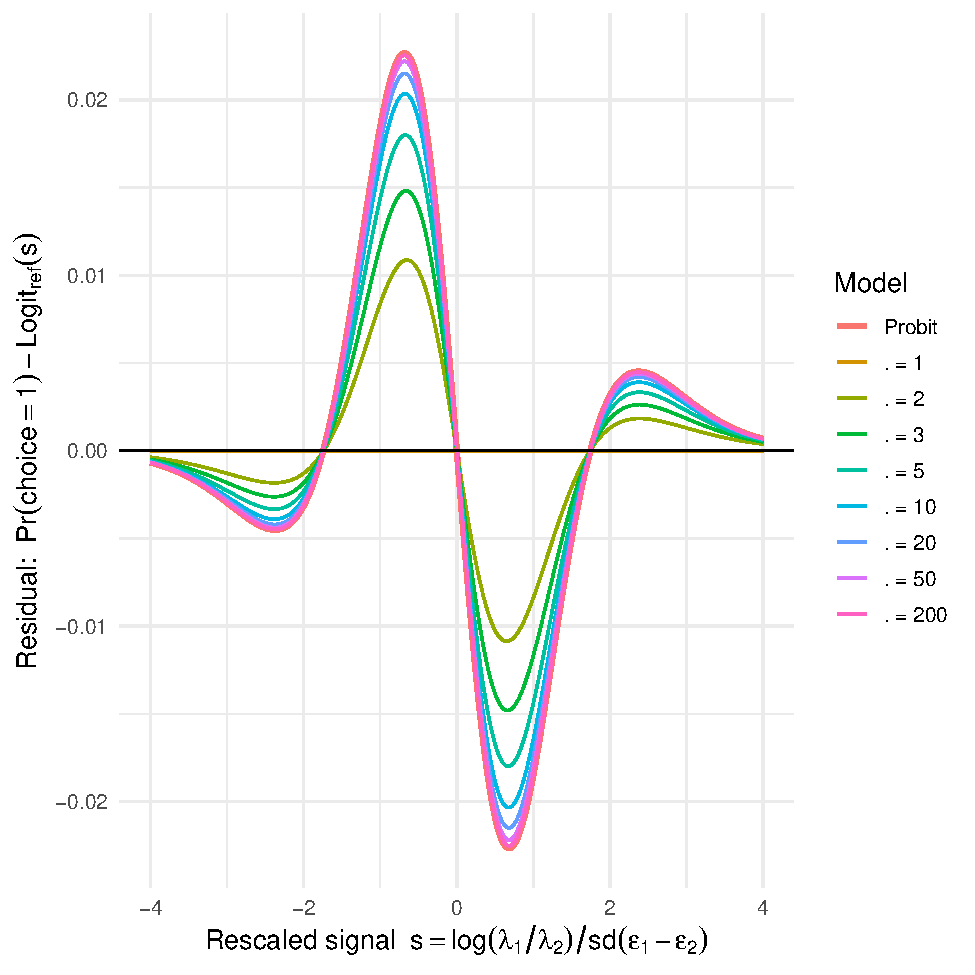
\includegraphics[keepaspectratio]{index_files/figure-pdf/fig-residuals-1.pdf}}

}

\end{figure}%

\textsubscript{Source:
\href{https://venpopov.github.io/logit-probit-poisson-rum/index.qmd.html}{Article
Notebook}}

\section{Simulation Studies: Multinomial K-alternative
Choice}\label{simulation-studies-multinomial-k-alternative-choice}

The binary simulation demonstrates that the variance-standardized
Poisson count race interpolates smoothly between Logit (\(\theta = 1\))
and Probit (\(\theta \to \infty\)) in the two-alternative case. Here I
extend this analysis to the multinomial setting (\(K > 2\)), where the
differences between logit and probit become richer and more
consequential.

In the binary case, logit and probit choice functions differ only in the
shape of the psychometric curve---a subtle quantitative distinction.
With three or more alternatives, additional qualitative differences
emerge. Most prominently, the Multinomial Logit model satisfies the
\emph{Independence of Irrelevant Alternatives} (IIA) property: the ratio
of choice probabilities for any two alternatives is independent of the
remaining alternatives in the choice set
(\citeproc{ref-luceIndividualChoiceBehavior1959}{Luce, 1959}). The
Multinomial Probit model, even with independent errors, does not share
this property (\citeproc{ref-hausmanConditionalProbitModel1978a}{Hausman
\& Wise, 1978}). The Poisson count race therefore provides a window into
how IIA-like behavior gradually weakens as the noise distribution
transitions from Gumbel to Gaussian.

The multinomial simulations are organised around five questions:

\begin{enumerate}
\def\labelenumi{\arabic{enumi}.}
\tightlist
\item
  \textbf{Convergence}: How quickly do Poisson count race choice
  probabilities converge to the Probit reference as \(\theta\)
  increases, and does the rate of convergence depend on \(K\)?
\item
  \textbf{Probability vectors}: How does the full distribution over
  alternatives change as \(\theta\) varies from 1 to large values?
\item
  \textbf{Set-size scaling}: How does the probability of choosing a
  target alternative scale with the number of competitors, and how does
  this scaling differ between logit, probit, and intermediate regimes?
\item
  \textbf{Independence of Irrelevant Alternatives}: How does the IIA
  property---exact under logit---erode as \(\theta\) increases toward
  the probit regime?
\item
  \textbf{Parameter invariance}: When misspecified logit or probit
  models are fit to Poisson count race data, which model yields
  parameters that are invariant to \(K\)?
\end{enumerate}

All simulations use Monte Carlo sampling with \(10^6\) to \(10^7\)
replications per condition unless otherwise noted.

\subsection{Study 1: Convergence to
Probit}\label{study-1-convergence-to-probit}

I first examine how the total variation (TV) distance between the
Poisson count race choice probabilities and the Logit / Probit
references changes as a function of \(\theta\), for different numbers of
alternatives \(K\).

For each \(K\), I use linearly spaced utilities
\(v_i = (K - i)/(K - 1)\) for \(i = 1, \ldots, K\), ensuring that the
best and worst alternatives always have utilities 1 and 0 regardless of
\(K\). The temperature is fixed at \(\beta = 1\).

\phantomsection\label{cell-fig-tv-distance}
\begin{figure}[H]

\caption{\label{fig-tv-distance}Total variation distance between Poisson
count race choice probabilities and the Logit (blue) and Probit (red)
references, as a function of threshold θ, for different numbers of
alternatives K.}

\centering{

\pandocbounded{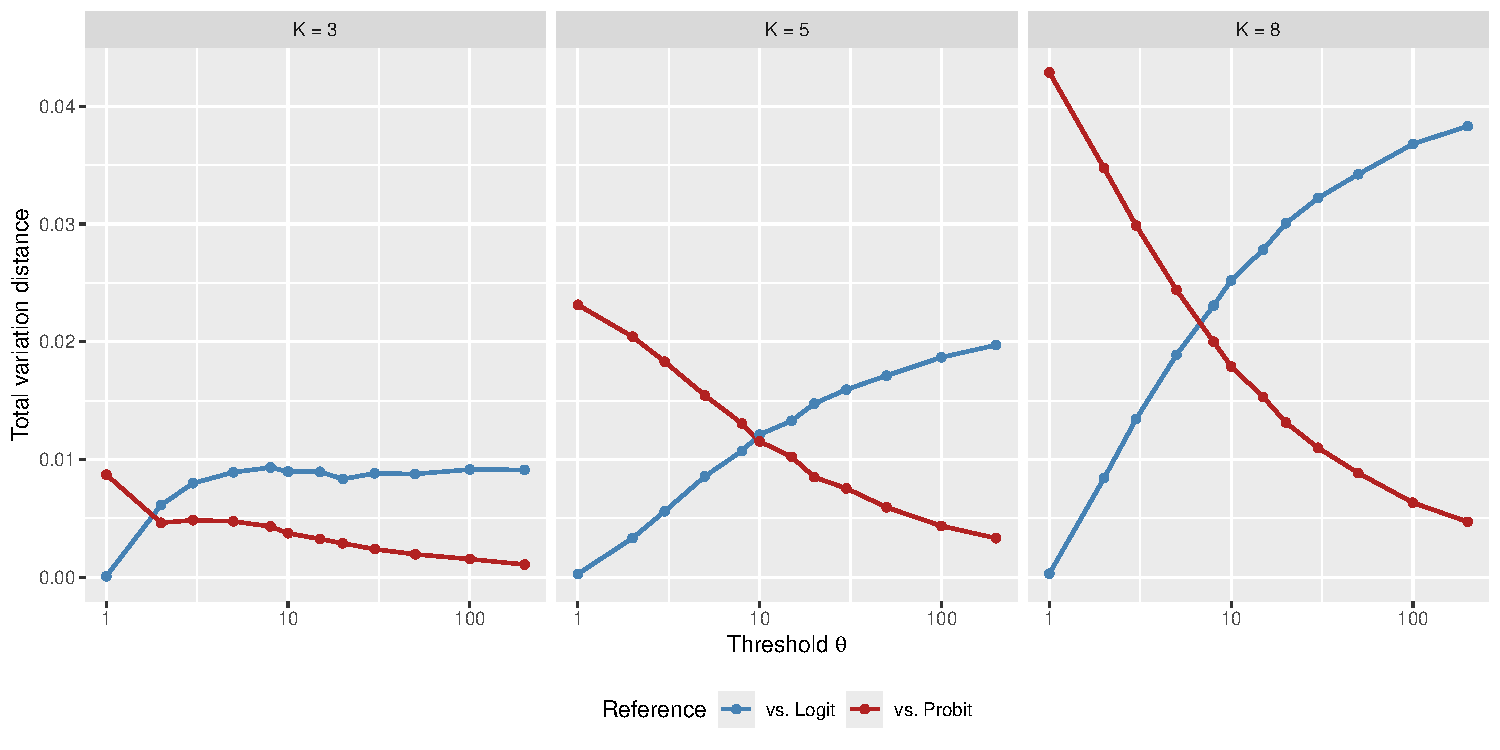
\includegraphics[keepaspectratio]{index_files/figure-pdf/fig-tv-distance-1.pdf}}

}

\end{figure}%

\textsubscript{Source:
\href{https://venpopov.github.io/logit-probit-poisson-rum/index.qmd.html}{Article
Notebook}}

\subsection{Study 2: Choice Probability
Vectors}\label{study-2-choice-probability-vectors}

To visualise how the full distribution over alternatives evolves with
\(\theta\), I fix \(K = 5\) with utilities
\(v = (2.0,\; 1.5,\; 1.0,\; 0.5,\; 0.0)\) and plot the choice
probability for each alternative across a range of thresholds.

\phantomsection\label{cell-fig-prob-vectors}
\begin{figure}[H]

\caption{\label{fig-prob-vectors}Choice probabilities for each of five
alternatives as a function of threshold θ. Dashed lines: Logit
reference; dotted lines: Probit reference.}

\centering{

\pandocbounded{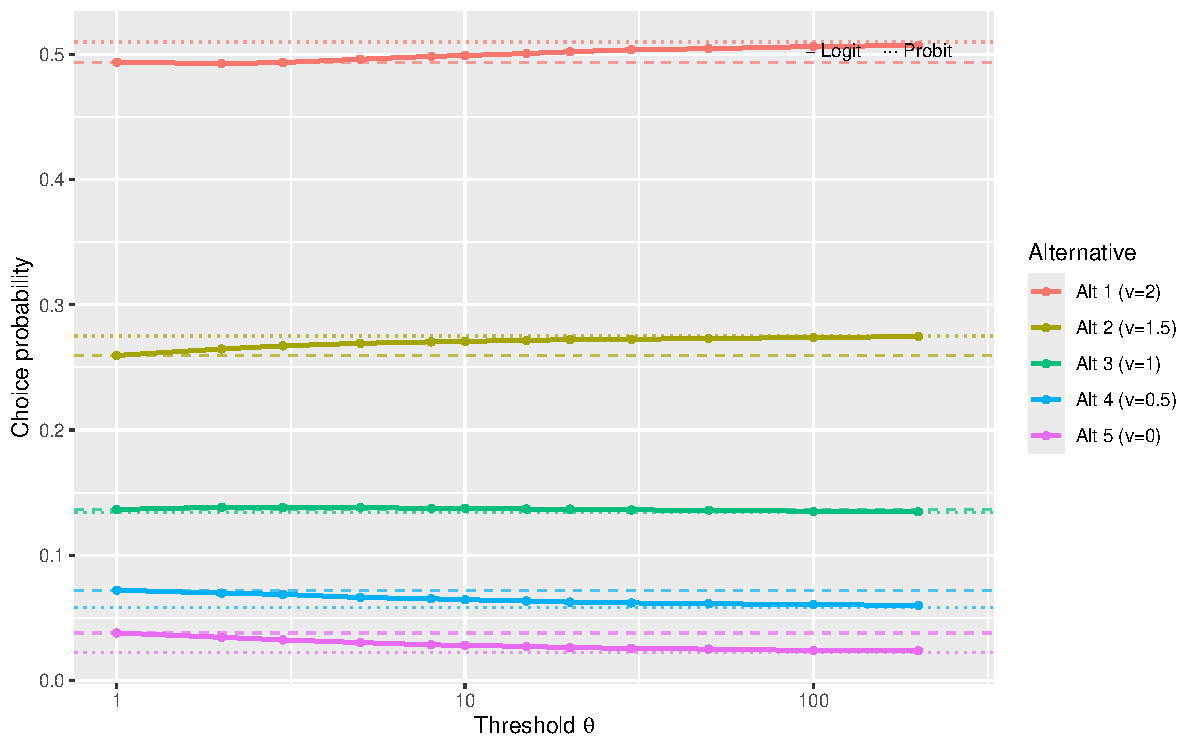
\includegraphics[keepaspectratio]{index_files/figure-pdf/fig-prob-vectors-1.pdf}}

}

\end{figure}%

\textsubscript{Source:
\href{https://venpopov.github.io/logit-probit-poisson-rum/index.qmd.html}{Article
Notebook}}

\subsection{Study 3: Set-Size Scaling}\label{study-3-set-size-scaling}

A critical diagnostic for discriminating between logit and probit models
is the effect of adding alternatives to the choice set
(\citeproc{ref-robinsonHowPeopleBuild2023}{Robinson et al., 2023}).
Under MNL, the probability of choosing a target alternative with fixed
utility is strictly determined by the ratio of its strength to the total
strength. Under MNP, the scaling with set size differs because the
probability of ``winning'' the maximum comparison depends on the shape
of the noise distribution.

I fix a target alternative with utility \(v_\text{target} = 1\) and add
\(K - 1\) equal competitors, each with utility \(v_\text{comp} = 0\). As
\(K\) grows, I track the probability of choosing the target.

Under MNL, the choice probability is
\(P(\text{target}) = e^a / (e^a + K - 1)\), where
\(a = v_t \cdot \pi / (\beta \sqrt{6})\) is the effective scaled
utility.

Under MNP:
\(P(\text{target}) = \int \phi(z) \,\Phi(v_t/\beta + z)^{K-1}\, dz\) (by
symmetry of the \(K - 1\) equal competitors). This integral reveals that
probit's thinner tails give the target a larger advantage over many
competitors than logit's heavier tails.

\phantomsection\label{cell-fig-set-size}
\begin{figure}[H]

\caption{\label{fig-set-size}Probability of choosing a target
alternative (v = 1) against K − 1 equal competitors (v = 0) as a
function of set size K. MNL (dashed blue) and MNP (dashed red)
references are shown.}

\centering{

\pandocbounded{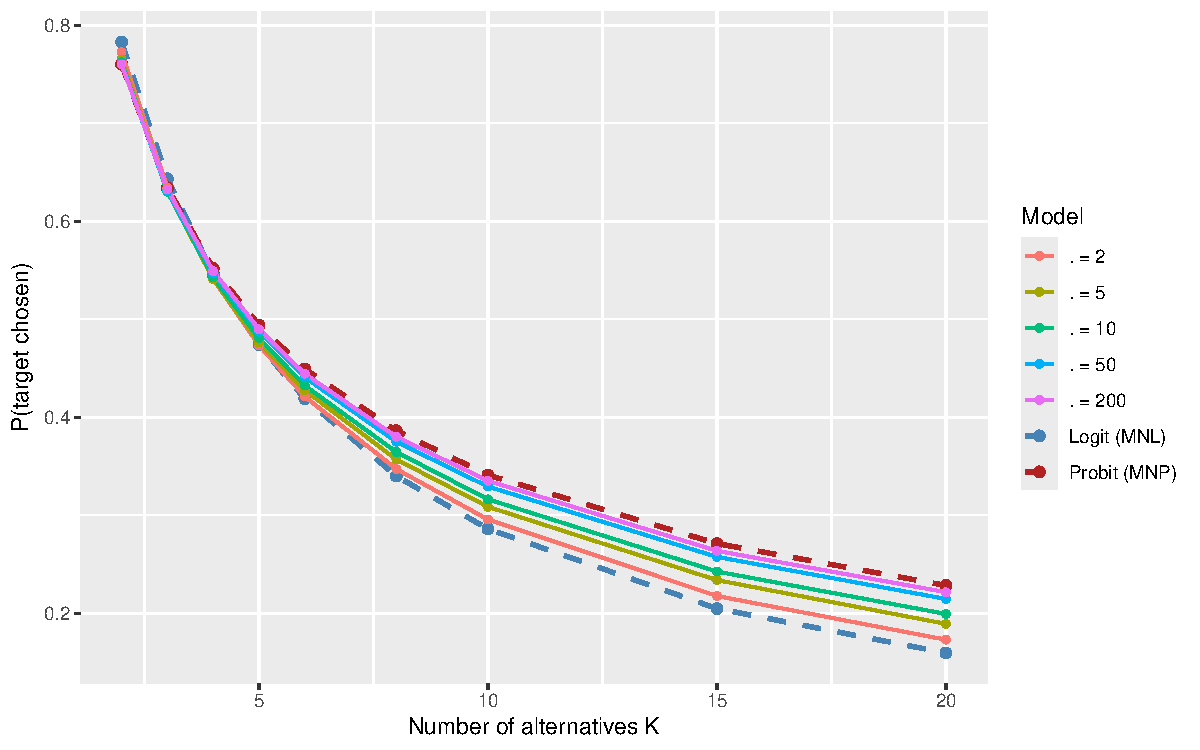
\includegraphics[keepaspectratio]{index_files/figure-pdf/fig-set-size-1.pdf}}

}

\end{figure}%

\textsubscript{Source:
\href{https://venpopov.github.io/logit-probit-poisson-rum/index.qmd.html}{Article
Notebook}}

\subsection{Study 4: Independence of Irrelevant
Alternatives}\label{study-4-independence-of-irrelevant-alternatives}

The IIA property is a hallmark of the Multinomial Logit model: the ratio
of choice probabilities for any two alternatives is invariant to the
composition of the choice set. Formally, for alternatives \(i\) and
\(j\):

\[\frac{P(i \mid \mathcal{C})}{P(j \mid \mathcal{C})} = \frac{e^{v_i}}{e^{v_j}} \quad \text{for all choice sets } \mathcal{C} \ni i, j\]

This property does not hold for the Multinomial Probit model, even when
errors are independent and identically distributed. The Poisson count
race therefore provides a mechanism through which IIA holds exactly at
\(\theta = 1\) and is progressively violated as \(\theta\) increases.

To quantify this, I consider three alternatives with utilities
\(v = (2, 1, 0)\). I compute the ratio \(P(1)/P(2)\) under two
conditions:

\begin{itemize}
\tightlist
\item
  \textbf{Full set}: all three alternatives present \(\{1, 2, 3\}\)
\item
  \textbf{Reduced set}: only alternatives \(\{1, 2\}\) present
\end{itemize}

Under IIA, these ratios should be identical. I track the percentage
change in the ratio as \(\theta\) varies.

\phantomsection\label{cell-fig-iia}
\begin{figure}[H]

\caption{\label{fig-iia}Test of IIA. Left: the ratio P(Alt 1)/P(Alt 2)
in the full set \{1, 2, 3\} (solid) and reduced set \{1, 2\} (dashed).
Right: percentage change in the ratio when alternative 3 is removed.}

\centering{

\pandocbounded{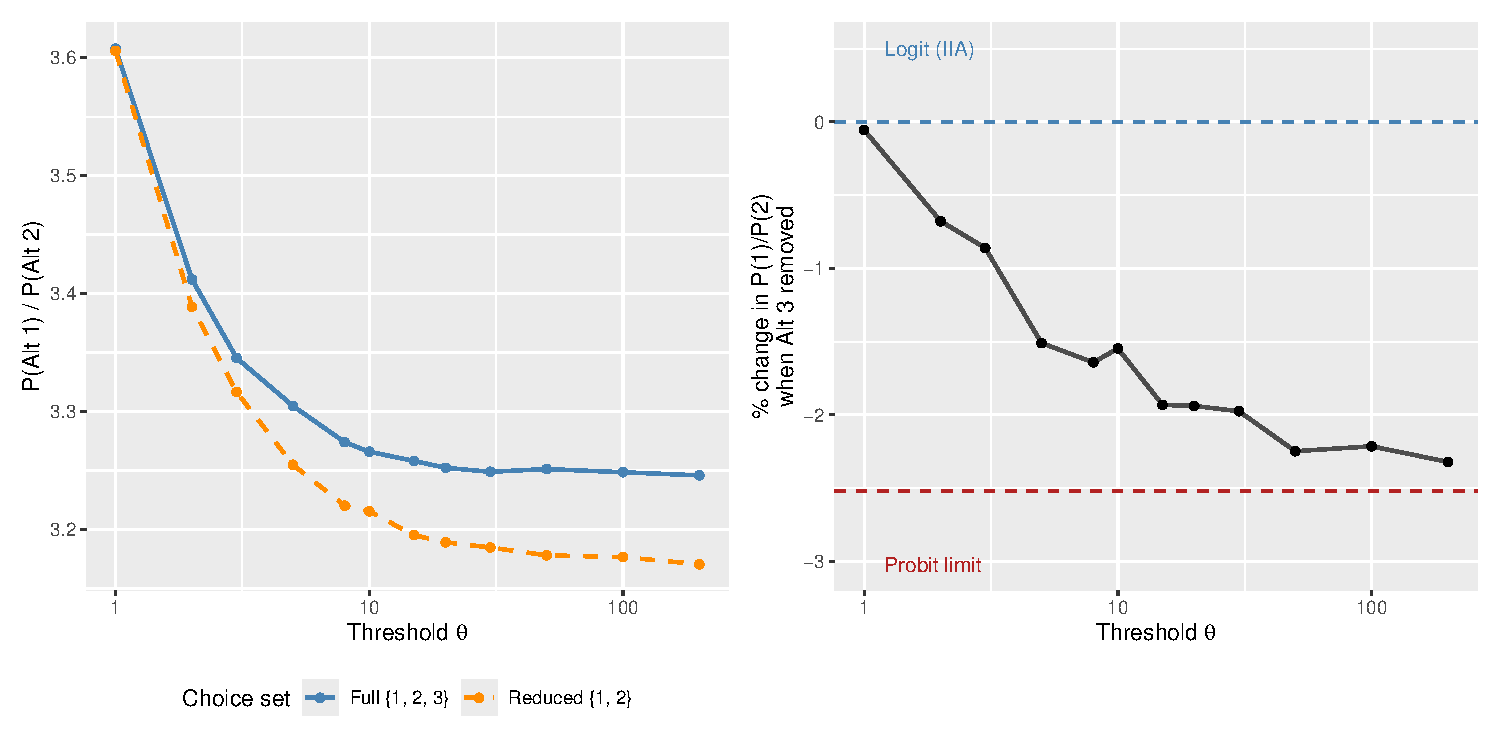
\includegraphics[keepaspectratio]{index_files/figure-pdf/fig-iia-1.pdf}}

}

\end{figure}%

\textsubscript{Source:
\href{https://venpopov.github.io/logit-probit-poisson-rum/index.qmd.html}{Article
Notebook}}

\subsection{Study 5: Parameter Invariance Across Set
Size}\label{study-5-parameter-invariance-across-set-size}

A key empirical diagnostic for distinguishing between logit and probit
is parameter invariance across changes in set size \(K\)
(\citeproc{ref-robinsonHowPeopleBuild2023}{Robinson et al., 2023}). If
choice data are generated by a logit model, the softmax inverse
temperature \(\beta_{\text{logit}}\) recovered from fitting a logit
specification should remain constant as \(K\) increases. Conversely, if
the data follow a probit model, the Gaussian noise scale
\(\beta_{\text{probit}}\) should be invariant to \(K\).

I test this directly. For each value of \(\theta\) and each set size
\(K\) (with a target at \(v = 1\) vs.~\(K-1\) equal competitors at
\(v = 0\)), I compute the ``true'' choice probability
\(P(\text{target})\) from the race model and then recover the
best-fitting logit and probit temperature parameters by inversion.

\phantomsection\label{cell-fig-parameter-recovery}
\begin{figure}[H]

\caption{\label{fig-parameter-recovery}Recovered temperature parameters
under logit (left) and probit (right) model assumptions as a function of
set size K and accumulation threshold θ.}

\centering{

\pandocbounded{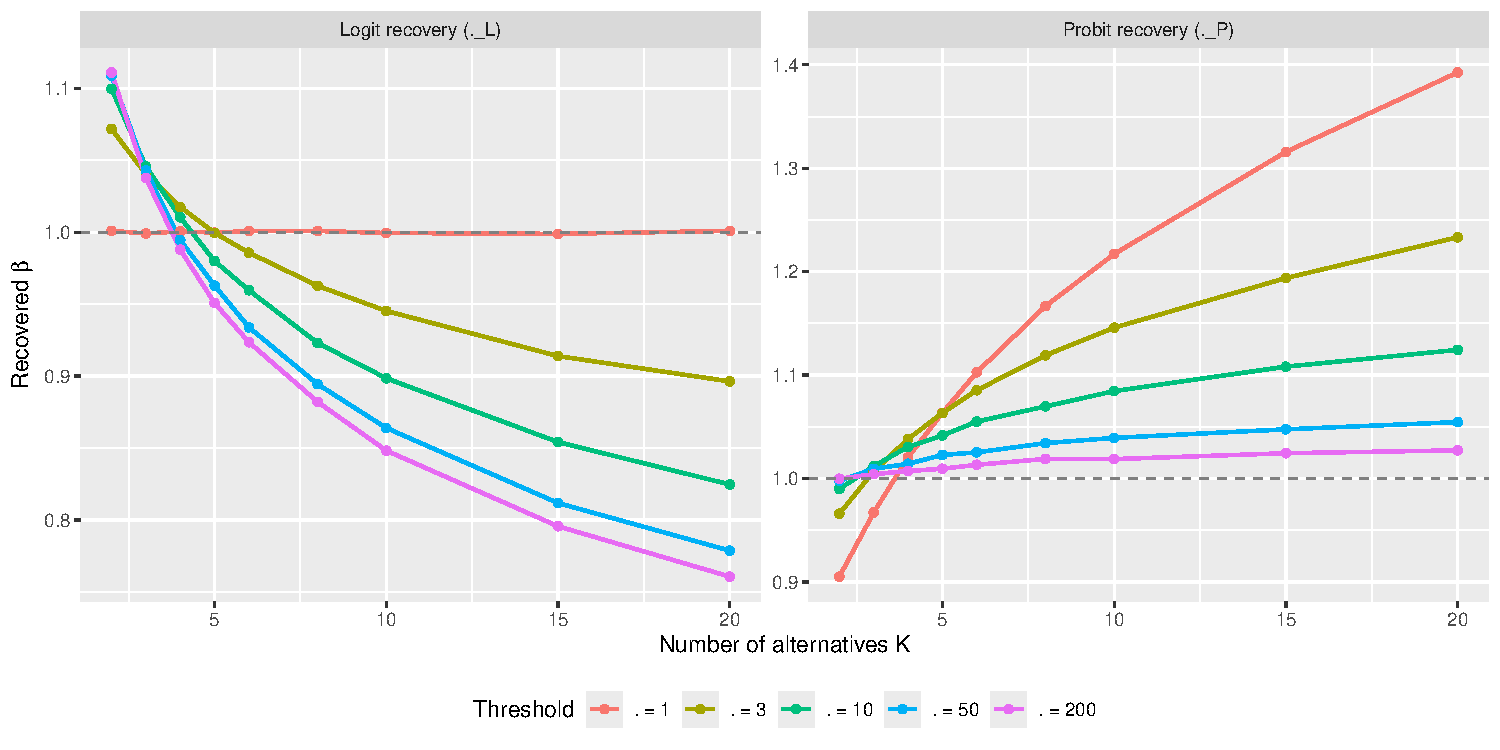
\includegraphics[keepaspectratio]{index_files/figure-pdf/fig-parameter-recovery-1.pdf}}

}

\end{figure}%

\textsubscript{Source:
\href{https://venpopov.github.io/logit-probit-poisson-rum/index.qmd.html}{Article
Notebook}}

\subsection{Study 6: Distributional Shape --- Noise Skewness and
Kurtosis}\label{study-6-distributional-shape-noise-skewness-and-kurtosis}

The log-Gamma noise distribution transitions from highly skewed (Gumbel,
\(\theta = 1\)) to symmetric (Gaussian, \(\theta \to \infty\)). This
transition in distributional shape underlies all the choice-level
phenomena documented above. To make this explicit, I plot the
standardised noise density for several values of \(\theta\) alongside
the standard normal reference.

\phantomsection\label{cell-fig-noise-densities}
\begin{figure}[H]

\caption{\label{fig-noise-densities}Standardised noise densities for
selected values of θ. As θ increases, the density converges to the
standard normal (black dashed).}

\centering{

\pandocbounded{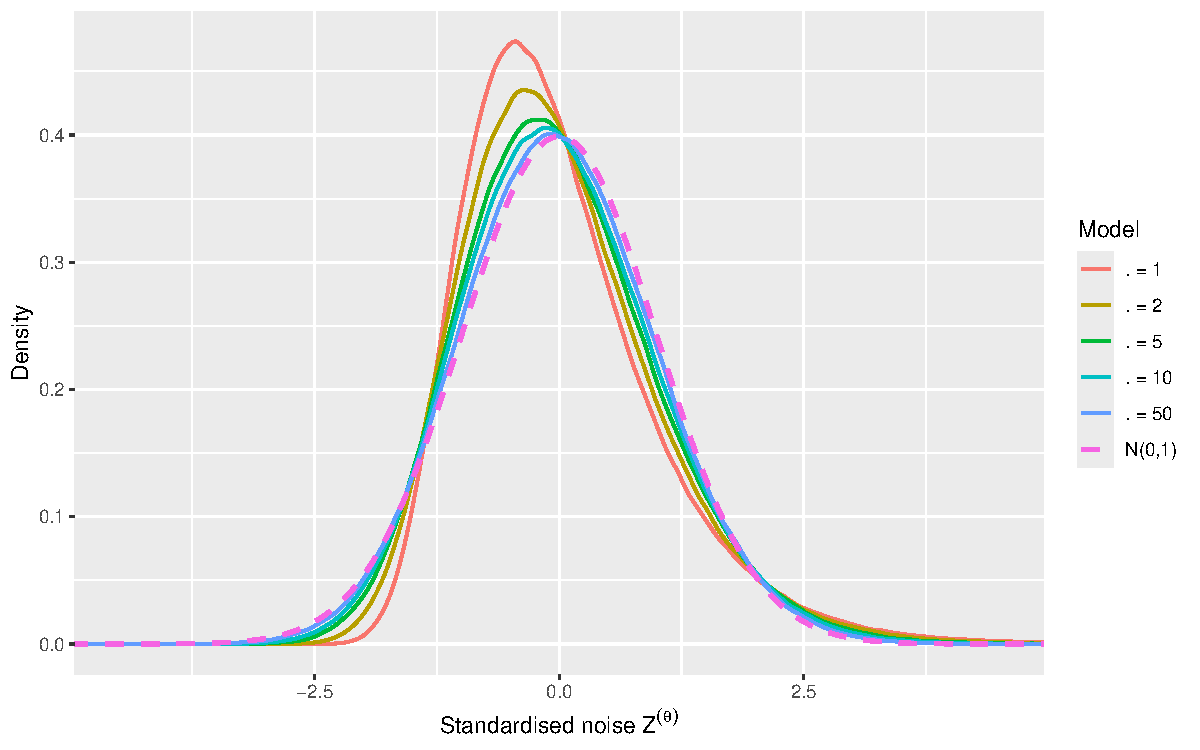
\includegraphics[keepaspectratio]{index_files/figure-pdf/fig-noise-densities-1.pdf}}

}

\end{figure}%

\textsubscript{Source:
\href{https://venpopov.github.io/logit-probit-poisson-rum/index.qmd.html}{Article
Notebook}}

\phantomsection\label{cell-fig-skew-kurtosis}
\begin{figure}[H]

\caption{\label{fig-skew-kurtosis}Skewness and excess kurtosis of the
standardised log-Gamma noise as a function of θ. Both moments converge
to zero (the Gaussian values) as θ increases, with skewness decaying as
O(θ\^{}\{-1/2\}) and excess kurtosis as O(θ\^{}\{-1\}). These moment
trajectories fully characterise the transition from Gumbel to Gaussian
noise shape.}

\centering{

\pandocbounded{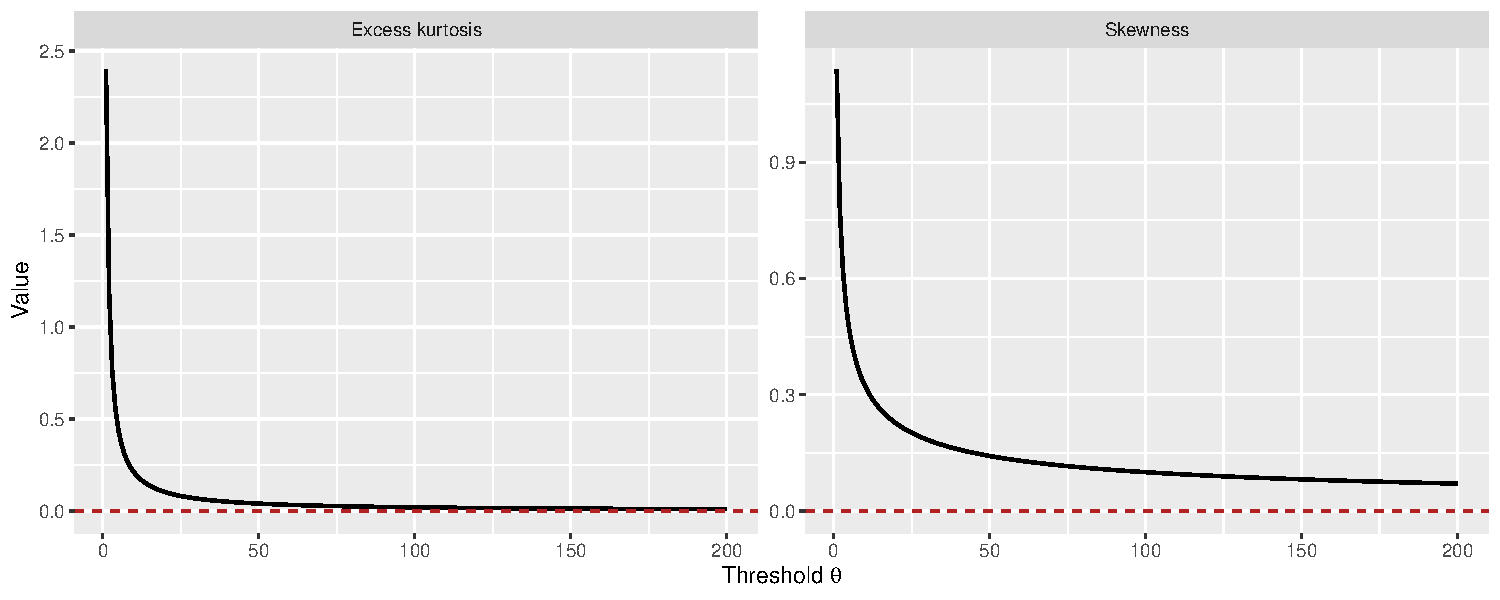
\includegraphics[keepaspectratio]{index_files/figure-pdf/fig-skew-kurtosis-1.pdf}}

}

\end{figure}%

\textsubscript{Source:
\href{https://venpopov.github.io/logit-probit-poisson-rum/index.qmd.html}{Article
Notebook}}

\subsection{Study 7: Robustness Across Utility
Structures}\label{study-7-robustness-across-utility-structures}

The preceding studies used specific utility vectors. To assess
robustness, I examine whether the convergence pattern holds across
different utility configurations that are common in psychological
experiments.

\phantomsection\label{cell-fig-robustness}
\begin{figure}[H]

\caption{\label{fig-robustness}Total variation distance from Probit as a
function of θ for K = 5 alternatives under four utility structures:
uniform, dominant, linear, and clustered.}

\centering{

\pandocbounded{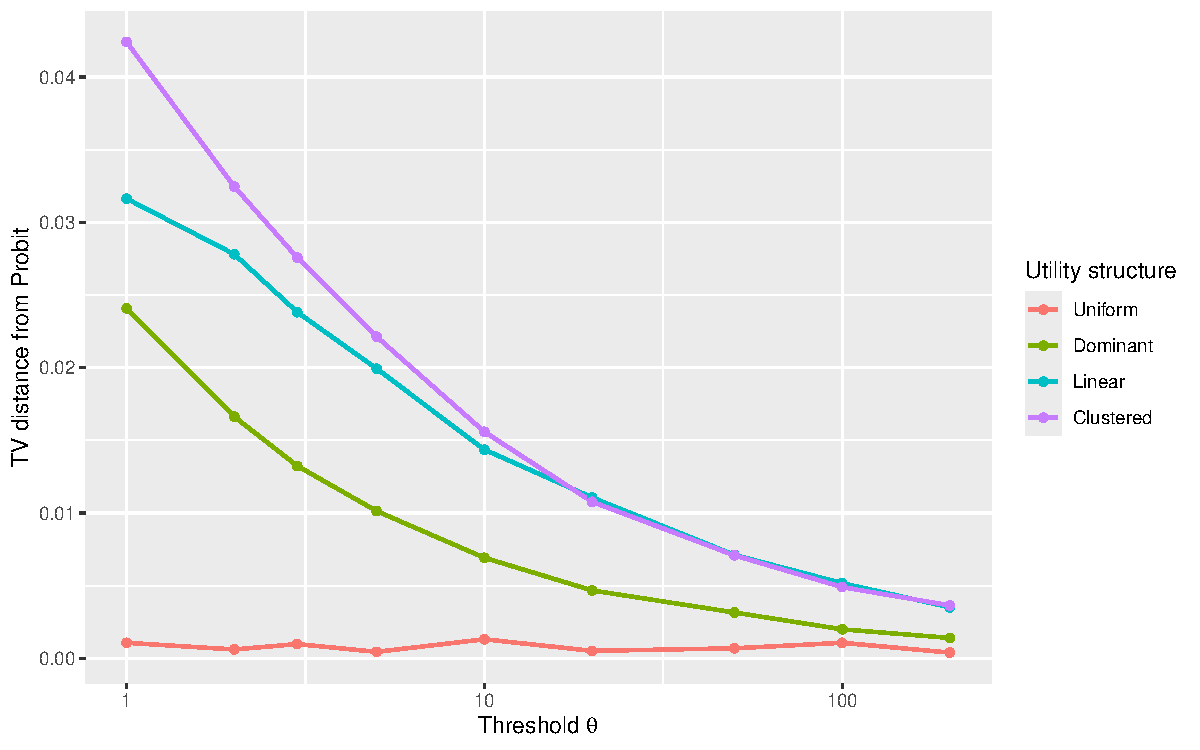
\includegraphics[keepaspectratio]{index_files/figure-pdf/fig-robustness-1.pdf}}

}

\end{figure}%

\textsubscript{Source:
\href{https://venpopov.github.io/logit-probit-poisson-rum/index.qmd.html}{Article
Notebook}}

\subsection{Summary}\label{summary}

These multinomial simulations confirm and extend the binary-case
results:

\begin{enumerate}
\def\labelenumi{\arabic{enumi}.}
\item
  \textbf{Convergence is gradual and universal}: Across different values
  of \(K\) and different utility structures, the Poisson count race
  converges to the Multinomial Probit reference within
  \(\theta \approx 50\)--\(100\) in total variation distance.
\item
  \textbf{Probability redistribution}: As \(\theta\) increases, the
  probit model concentrates more probability on the best alternative and
  less on inferior alternatives, reflecting the thinner tails of
  Gaussian noise relative to Gumbel.
\item
  \textbf{Set-size scaling}: The logit and probit models predict
  systematically different scaling of target choice probability with the
  number of competitors. The Poisson count race interpolates between
  these two patterns, connecting to the empirical findings of
  (\citeproc{ref-robinsonHowPeopleBuild2023}{Robinson et al., 2023}).
\item
  \textbf{IIA erosion}: The Independence of Irrelevant Alternatives
  property, which holds exactly at \(\theta = 1\), is progressively
  violated as \(\theta\) increases. This provides a process-level
  account of why IIA holds for logit but not probit: it is a consequence
  of the Gumbel noise shape, and alternative noise shapes---induced by
  higher accumulation thresholds---do not preserve it.
\item
  \textbf{Parameter invariance}: When choice data generated by the
  Poisson count race are fit under a logit assumption, the recovered
  inverse temperature drifts with set size \(K\) for all \(\theta > 1\).
  Conversely, when fit under a probit assumption, the recovered noise
  scale remains stable for large \(\theta\) but drifts when \(\theta\)
  is small. This cross-over in parameter invariance provides a
  process-level account of the empirical findings of
  (\citeproc{ref-robinsonHowPeopleBuild2023}{Robinson et al., 2023}):
  parameter stability across \(K\) is diagnostic of whether the
  effective noise distribution is closer to Gumbel or Gaussian.
\item
  \textbf{Noise shape transition}: The underlying mechanism is a smooth
  transition in the shape of the standardised noise distribution, from
  the skewed Gumbel (\(\theta = 1\)) to the symmetric Gaussian
  (\(\theta \to \infty\)). The skewness and kurtosis decay at known
  rates, providing analytic control over the approximation quality.
\end{enumerate}

\section{Extending the Race Model to Correlated
Errors}\label{extending-the-race-model-to-correlated-errors}

The core model described thus far restricts the underlying count
processes to be strictly independent, yielding the Independent
Multinomial Probit in the asymptotic limit. However, the primary
theoretical appeal of probit models lies in their ability to accommodate
correlated error structures, thereby capturing similarity effects and
systematic violations of the Independence of Irrelevant Alternatives
(IIA). In this section, I demonstrate that the Poisson count race can be
naturally extended to generate the full Correlated Multinomial Probit by
introducing shared evidence generators. This provides a mechanistic,
process-level account for how covariance structures emerge in static
choice models.

\subsection{The Shared-Feature
Mechanism}\label{the-shared-feature-mechanism}

To induce correlation without violating the stationary, independent
increments of the individual Poisson generators, we abandon the
assumption that all events are strictly unique to a specific
alternative. Instead, we define a multivariate Poisson process
representing ``features'' or ``shocks'' that alternatives can share.

Let \(S \subseteq \{1, \dots, K\}\) denote a subset of alternatives.
Assume the existence of independent feature generators \(Y_S(t)\), which
are Poisson processes with rates \(\lambda_S \ge 0\). An event from
\(Y_S(t)\) delivers a simultaneous unit of evidence to all alternatives
contained in \(S\). The cumulative count for alternative \(i\) is the
superposition of all feature processes associated with it:

\[N_i(t) = \sum_{S: i \in S} Y_S(t)\]

Because the superposition of independent Poisson processes is itself a
Poisson process, \(N_i(t)\) remains a standard Poisson process with
marginal rate \(\Lambda_i = \sum_{S: i \in S} \lambda_S\). The waiting
time marginals are therefore preserved as
\(T_i^{(\theta)} \sim \text{Gamma}(\theta, \Lambda_i)\).

Crucially, for any two alternatives \(i\) and \(j\) that share at least
one feature generator, their event counts covary. The covariance is
determined by the sum of the rates of their shared processes:

\[\text{Cov}(N_i(t), N_j(t)) = t \sum_{S: \{i,j\} \subseteq S} \lambda_S := t \Lambda_{ij}\]

This yields a correlation between the accumulators of
\(\rho_{ij} = \Lambda_{ij} / \sqrt{\Lambda_i \Lambda_j}\).

\subsection{The Correlated Probit
Limit}\label{the-correlated-probit-limit}

To find the asymptotic joint distribution of the choice model, we apply
the Multivariate Central Limit Theorem for the multivariate Poisson
counting process. As \(\theta \to \infty\), the standardized hitting
times jointly converge to a Multivariate Normal distribution.

Applying the utility transformation
\(U_i^{(\theta)} = \log \Lambda_i - \log G_i\), where
\(G_i = \Lambda_i T_i^{(\theta)}\) is marginally
\(\text{Gamma}(\theta, 1)\) but now correlated across alternatives, and
the Multivariate Delta Method (with \(g(x) = -\log x\)), the
unstandardized random utility errors converge to a Multivariate Normal
distribution whose covariance scales as
\(\psi_1(\theta) \rho_{ij} \approx (1/\theta)\rho_{ij}\).

When we apply the variance normalization from Section 4 to enforce
matched discriminability, we define the standardized noise
\(Z_i^{(\theta)} = (\epsilon_i^{(\theta)} - \mu_\theta) / \sigma_\theta\).
Because
\(\sigma_\theta = \sqrt{\psi_1(\theta)} \approx 1/\sqrt{\theta}\) for
large \(\theta\), dividing the covariance by
\(\sigma_\theta^2 = \psi_1(\theta)\) exactly recovers \(\rho_{ij}\). The
standardized noise vector \(\mathbf{Z}^{(\theta)}\) thus converges in
distribution to a multivariate standard normal with the correlation
matrix of the underlying counting processes:

\[\mathbf{Z}^{(\theta)} \xrightarrow{d} \mathcal{N}(\mathbf{0}, \mathbf{R})\]

where \(\mathbf{R}\) has off-diagonal elements \(\rho_{ij}\).
Consequently, the random utility vector converges to
\(\mathbf{U}^{(\theta)} \xrightarrow{d} \mathcal{N}(\mathbf{v}, \beta^2 \mathbf{R})\).
This establishes the shared-feature Poisson count race as a valid
generative foundation for the full Correlated Multinomial Probit.

\subsection{Variance Normalization and Parameter
Recovery}\label{variance-normalization-and-parameter-recovery}

While the asymptotic proof establishes the theoretical limit, analyzing
the behavior of the shared-feature model under the variance
normalization introduced in Section 4 reveals critical boundary
conditions of evidence accumulation.

To maintain matched discriminability across varying thresholds
\(\theta\), the systematic utilities \(v_i\) must remain constant while
the noise is scaled. Because the systematic utility in the
unstandardized race is \(\log(\Lambda_i)\), the \emph{effective total
rates} must scale with \(\sigma_\theta = \sqrt{\psi_1(\theta)}\):

\[\Lambda_i^* = \exp(v_i \sigma_\theta)\]

Consider a two-alternative scenario where options 1 and 2 share a
feature generator with rate \(\lambda_{12}^*\), and possess unique
generators with rates \(\lambda_1^*\) and \(\lambda_2^*\). To achieve a
target correlation \(\rho\), the shared rate must be:

\[\lambda_{12}^* = \rho \sqrt{\Lambda_1^* \Lambda_2^*} = \rho \exp\left(\frac{(v_1 + v_2) \sigma_\theta}{2}\right)\]

The required unique rate for alternative 2 is therefore
\(\lambda_2^* = \Lambda_2^* - \lambda_{12}^*\). For the model to be
physically coherent as a Poisson process, this unique rate must be
strictly non-negative (\(\lambda_2^* \ge 0\)).

\subsection{A Mechanistic Account of Substitution and Boundary
Conditions}\label{a-mechanistic-account-of-substitution-and-boundary-conditions}

This non-negativity constraint provides a concrete process-level
explanation for substitution effects. If alternative 1 is vastly
superior to alternative 2 (\(v_1 \gg v_2\)), and the correlation
\(\rho\) is high, nearly all events that provide evidence for the weaker
alternative are \emph{shared} events that simultaneously provide
evidence for the stronger alternative. The stronger alternative
``cannibalizes'' the probability mass of the weaker option because it
possesses a robust unique evidence stream, while the weaker option
possesses almost none.

Mathematically, ensuring \(\lambda_2^* \ge 0\) reveals a strict upper
bound on the correlation the system can support for a given threshold
and utility difference. Dividing by \(\Lambda_2^*\), we find:

\[\rho_{\max} = \exp\left(-\frac{(v_1 - v_2) \sigma_\theta}{2}\right)\]

This equation demonstrates that in a physical evidence accumulation
system, correlation and utility are not entirely independent parameters.
A decision-maker operating at a low threshold \(\theta\) (where
\(\sigma_\theta\) is large) structurally cannot sustain highly
correlated representations of asymmetric options without the weaker
option's unique evidence stream collapsing below zero. However, as the
decision-maker becomes more cautious (\(\theta \to \infty\)), the
scaling factor \(\sigma_\theta \to 0\), and \(\rho_{\max} \to 1\). The
theoretical limit seamlessly supports arbitrary correlation matrices,
but the generative mechanics reveal that high correlation between
disparate utilities requires prolonged, thresholded accumulation.

\subsection{The Cost of Covariance: Degeneracy at the Logit
Boundary}\label{the-cost-of-covariance-degeneracy-at-the-logit-boundary}

While independent accumulators provide a smooth, continuous bridge from
the Multinomial Logit (\(\theta=1\)) to the Independent MNP
(\(\theta \to \infty\)), the introduction of shared features
fundamentally breaks the isomorphism at the Logit boundary.

At \(\theta=1\), a shared event \(Y_S(t)\) reaching the single-count
threshold causes simultaneous crossing for multiple alternatives. This
results in a tie, violating the continuous distribution assumption
necessary to derive the Luce choice rule from Extreme Value Theory and
necessitating arbitrary discrete tie-breaking.

Furthermore, because incorporating a target correlation \(\rho\)
requires dynamically shifting probability mass into the shared generator
\(\lambda_{12}^*\), the first two moments (variance and covariance) of
the utility distribution are fixed by the target covariance structure
across all \(\theta\). Consequently, the choice probabilities exhibit
Probit-like substitution patterns at all thresholds, not only in the
asymptotic limit. Thus, while independent accumulators trace the
transition of noise \emph{shape} from Gumbel to Gaussian, shared
accumulators sacrifice this interpolation to map the generative model
onto the exact covariance structures required for general discrete
choice applications.

\section{Discussion}\label{discussion}

The present work develops a generative framework in which Multinomial
Logit and Multinomial Probit arise as endpoint regimes of a single
parametric family of stochastic accumulation models. By introducing a
Poisson count race and a variance standardization that separates noise
scale from noise shape, this paper clarifies how extreme-value and
Gaussian choice behavior emerge as members of the log-Gamma random
utility family, indexed by the accumulation threshold \(\theta\). As
discussed in Section 5, this bridge is distributional rather than
dynamical: the variance standardization compares different accumulation
systems at matched discriminability, rather than describing the behavior
of a single system under threshold manipulation. The goal is not to
advocate replacing existing models, but to clarify their relationship:
logit and probit represent different positions within a continuum of
log-Gamma noise shapes, with the accumulation threshold governing the
transition between them.

The multinomial simulations demonstrate that this unification is not
merely a theoretical curiosity. Thresholded accumulation induces
systematic, graded violations of IIA that converge toward the dependence
structure characteristic of multinomial probit. This dependence emerges
endogenously from the accumulation and stopping rule, rather than being
imposed by construction. The parameter invariance results further
connect the framework to recent empirical findings
(\citeproc{ref-robinsonHowPeopleBuild2023}{Robinson et al., 2023}),
providing a process-level account of why Gaussian-based parameters
exhibit greater stability across changes in set size.

\subsection{Relation to existing
models}\label{relation-to-existing-models}

From a mathematical standpoint, all components of the present framework
are classical: exponential races yield Luce's choice rule, Gamma waiting
times arise from accumulated Poisson events, and asymptotic normality
follows from the Central Limit Theorem. The contribution lies in
assembling these elements into a single generative family and
identifying the conditions under which its limiting behavior remains
non-degenerate.

The present model should not be conflated with full sequential sampling
models such as the Diffusion Decision Model
(\citeproc{ref-ratcliffTheoryMemoryRetrieval1978}{Ratcliff, 1978}) or
Linear Ballistic Accumulator
(\citeproc{ref-brownBallisticModelChoice2005}{Brown \& Heathcote,
2005}). Those models jointly account for response times and accuracy via
continuous accumulation with explicit drift and boundary parameters. The
Poisson count race is deliberately minimal: it uses accumulation as a
generative device to induce a family of random utility models, without
making claims about within-trial dynamics or response time
distributions.

Between the logit and probit endpoints lies a continuum of log-Gamma
random utility models. These intermediate regimes are not intended as
new default specifications, but they underscore that logit and probit
are special cases of a broader family. Deviations from logit or probit
behavior may sometimes reflect differences in accumulation thresholds
rather than fundamentally different noise sources.

\subsection{Implications for empirical
modeling}\label{implications-for-empirical-modeling}

The present framework offers a theoretical account of why logit-based
and probit-based models may differ in parameter invariance across task
structures. Models with larger effective accumulation thresholds
naturally exhibit Gaussian-like behavior, which may confer greater
stability across changes in the number of alternatives. At the same
time, the results caution against interpreting superior empirical
performance of one model class as evidence for a particular noise
distribution in isolation: differences between logit and probit may
reflect differences in decision criteria or commitment thresholds rather
than differences in representational noise per se.

\subsection{Limitations and
extensions}\label{limitations-and-extensions}

The Poisson count race is intentionally simple and focuses exclusively
on choice probabilities, abstracting away from response times and
within-trial dynamics. Although the shared-feature extension developed
in the preceding section demonstrates how correlated accumulators can
generate the full Correlated Multinomial Probit, additional extensions
such as time-varying rates or joint modeling of choice and response time
are natural directions for future work.

The present analysis treats the accumulation threshold as fixed across
trials and alternatives. Allowing threshold variability or adaptive
stopping rules could further enrich the family of induced choice models
and connect more directly to theories of decision caution and
speed--accuracy trade-offs.

The model positions the Poisson count race as a parametric family
indexed by \((\theta, \beta)\), but a formal identification analysis is
beyond the present scope. In principle, \(\theta\) and \(\beta\) play
distinct roles---shape versus scale of the noise distribution---and the
shape of the psychometric function or the pattern of IIA violations
could serve to identify \(\theta\) from choice data. Whether these
parameters are jointly identifiable from aggregate choice frequencies
alone, and under what experimental designs, remains an open question for
future investigation.

Finally, the framework naturally invites comparison with other random
utility specifications. Exploring whether additional classical models
arise as limiting regimes under alternative accumulation rules may
provide further insight into the structure of discrete choice behavior.

\subsection{Concluding remarks}\label{concluding-remarks}

By grounding discrete choice models in a common stochastic accumulation
process, the Poisson count race reframes a long-standing modeling
distinction. Logit and probit emerge not as competing assumptions about
utility noise, but as members of a single parametric family --- the
log-Gamma random utility models --- indexed by the accumulation
threshold \(\theta\). This unification is algebraic and distributional:
it reveals that the two canonical specifications occupy endpoint
positions within a continuous family of noise shapes, rather than
representing fundamentally distinct generating mechanisms. At the same
time, the unification does not imply that a single decision system can
transition between regimes by adjusting its threshold alone, since the
variance standardization that enables comparison across \(\theta\)
values entails different effective rate structures. The framework thus
clarifies the conceptual relationship between logit and probit and
provides a principled basis for comparison, illustrating how
process-level reasoning can illuminate the structure of static choice
models.

\section{References}\label{references}

\phantomsection\label{refs}
\begin{CSLReferences}{1}{0}
\bibitem[\citeproctext]{ref-brownBallisticModelChoice2005}
Brown, S., \& Heathcote, A. (2005). A {Ballistic Model} of {Choice
Response Time}. \emph{Psychological Review}, \emph{112}(1), 117--128.
\url{https://doi.org/10.1037/0033-295X.112.1.117}

\bibitem[\citeproctext]{ref-falmagneRepresentationTheoremFinite1978a}
Falmagne, J. C. (1978). A representation theorem for finite random scale
systems. \emph{Journal of Mathematical Psychology}, \emph{18}(1),
52--72. \url{https://doi.org/10.1016/0022-2496(78)90048-2}

\bibitem[\citeproctext]{ref-hausmanConditionalProbitModel1978a}
Hausman, J. A., \& Wise, D. A. (1978). A {Conditional Probit Model} for
{Qualitative Choice}: {Discrete Decisions Recognizing Interdependence}
and {Heterogeneous Preferences}. \emph{Econometrica}, \emph{46}(2),
403--426. \url{https://doi.org/10.2307/1913909}

\bibitem[\citeproctext]{ref-kellenTestingFoundationsSignal2021}
Kellen, D., Winiger, S., Dunn, J. C., \& Singmann, H. (2021). Testing
the foundations of signal detection theory in recognition memory.
\emph{Psychological Review}, \emph{128}(6), 1022--1050.
\url{https://doi.org/10.1037/rev0000288}

\bibitem[\citeproctext]{ref-luceIndividualChoiceBehavior1959}
Luce, R. D. (1959). \emph{Individual choice behavior} (pp. xii, 153).
John Wiley.

\bibitem[\citeproctext]{ref-mcfaddenConditionalLogitAnalysis1974}
McFadden, D. (1974). Conditional logit analysis of qualitative choice
behavior. In \emph{Frontiers in econometrics} (p. 105).

\bibitem[\citeproctext]{ref-pikeResponseLatencyModels1973}
Pike, R. (1973). Response latency models for signal detection.
\emph{Psychological Review}, \emph{80}(1), 53--68.
\url{https://doi.org/10.1037/h0033871}

\bibitem[\citeproctext]{ref-ratcliffTheoryMemoryRetrieval1978}
Ratcliff, R. (1978). A theory of memory retrieval. \emph{Psychological
Review}, \emph{85}(2), 59--108.
\url{https://doi.org/10.1037/0033-295X.85.2.59}

\bibitem[\citeproctext]{ref-robinsonHowPeopleBuild2023}
Robinson, M. M., DeStefano, I. C., Vul, E., \& Brady, T. F. (2023). How
do people build up visual memory representations from sensory evidence?
{Revisiting} two classic models of choice. \emph{Journal of Mathematical
Psychology}, \emph{117}, 102805.
\url{https://doi.org/10.1016/j.jmp.2023.102805}

\bibitem[\citeproctext]{ref-smithTimedependentPoissonCounter2000a}
Smith, P. L., \& Van Zandt, T. (2000). Time-dependent {Poisson} counter
models of response latency in simple judgment. \emph{British Journal of
Mathematical and Statistical Psychology}, \emph{53}(2), 293--315.
\url{https://doi.org/10.1348/000711000159349}

\bibitem[\citeproctext]{ref-thurstoneLawComparativeJudgment1927}
Thurstone, L. L. (1927). A law of comparative judgment.
\emph{Psychological Review}, \emph{34}(4), 273--286.
\url{https://doi.org/10.1037/h0070288}

\bibitem[\citeproctext]{ref-townsendStochasticModelingElementary1983}
Townsend, J. T., \& Ashby, F. G. (1983). \emph{The stochastic modeling
of elementary psychological processes}. Cambridge University Press.

\bibitem[\citeproctext]{ref-wixtedForgottenHistorySignal2020}
Wixted, J. T. (2020). The forgotten history of signal detection theory.
\emph{Journal of Experimental Psychology: Learning, Memory, and
Cognition}, \emph{46}(2), 201--233.
\url{https://doi.org/10.1037/xlm0000732}

\bibitem[\citeproctext]{ref-yellottRelationshipLucesChoice1977}
Yellott, J. (1977). The relationship between {Luce}'s {Choice Axiom},
{Thurstone}'s {Theory} of {Comparative Judgment}, and the double
exponential distribution. \emph{Journal of Mathematical Psychology},
\emph{15}(2), 109--144.
\url{https://doi.org/10.1016/0022-2496(77)90026-8}

\end{CSLReferences}






\end{document}
